\documentclass{article}
\usepackage[utf8]{inputenc}
\usepackage{amsmath}
\usepackage{natbib}
\linespread{1}
\usepackage{bm}
\usepackage{mcode}
\usepackage[lighttt]{lmodern}
\usepackage{graphicx} 
\usepackage{epstopdf}
\usepackage{algorithm2e}
\usepackage{multicol}
\usepackage{float}
\usepackage{subfigure}
\title{\LARGE{Polymer Chain Dynamics Simulation}\\ \large{Report}
}
\author{ZHA Chenyu}
%\date{5.Mars.2015}
\renewcommand*\contentsname{Table de matière}

\begin{document}

\maketitle
\pagebreak


\section{The random walk model:the freely jointed chain}
\paragraph{}

Consider a linear polymer to be a freely-jointed chain with N beads, length of each bond is $b$ , that occupy zero volume. The path of the chains is like a 'random walk 'in three dimensions, limited only by the constraint that each segment must be joined to its neighbors.\\

Consider the 'end to end' vector $\bm{R}$ joining one end of the polymer to the other,the average value $<\bm{R}>$ is zero,since the probability of R equals -R.Therefore we will calculate $<\bm{R^2}>$
\begin{equation}
<\bm{R^2}>=\sum_{{n=1}}^{N}\sum_{m=1}^{N}<r_n\cdot r_m>
\end{equation} 
We consider that there is no correlation between bead $n$ and $m$,therefore we find :
\begin{equation}
<\bm{R^2}>=\sum_{{n=1}}^{N}<r_n^2>=Nb^2
\end{equation}
The probability distribution of $\bm{R}$ is:
\begin{equation}
P(\bm{R},N)=(\frac{3}{2\pi Nb^2})^{3/2}exp(-\frac{3\bm{R}^2}{2Nb^2})
\end{equation}
The probability distribution function of $\bm{R}$ obeys the Gaussian distribution.
The position of the beads after each step will satisfy the diffusion equation :
\begin{equation}
\bm{R(t+\Delta t)}=\bm{R(t)}+\sqrt{2D\Delta t}\bm{g(t)}
\end{equation}
$\bm{g(t)}$ is normally distributed random noise.
\subsection{Random walk Simulation}
\begin{lstlisting}
%This program is used to simulate the brownian motion
classdef FirstTry<handle

properties
dimension%dimension=1,2 or 3
numParticles%number of particles in polymers;
dt%pas de temps
numSteps% number of motion
diffusionConst %constante diffusion
paths %the paths of polymer;
end

methods

%class constructor
function obj=FirstTry(dimension,numParticles,dt,diffusionConst,numSteps)
obj.dimension=dimension;
obj.numParticles=numParticles;
obj.dt=dt;
obj.numSteps=numSteps;
obj.diffusionConst=diffusionConst;
obj.paths = zeros(obj.numParticles,3,obj.numSteps);
end


function Calculate(obj)

for j=1
noise = [zeros(1,obj.dimension);...
sqrt(2*obj.diffusionConst*obj.dt)*randn(obj.numParticles-1,obj.dimension)];
obj.paths(:,1:obj.dimension,j)=cumsum(noise);

end

for j=2:obj.numSteps
noise = [sqrt(2*obj.diffusionConst*obj.dt)*randn(obj.numParticles,obj.dimension)];
obj.paths(:,1:obj.dimension,j)=obj.paths(:,1:obj.dimension,j-1)+noise;

end


end %'random walk 'simulation

function Plot(obj)
f=figure;
b =[-20 20];
a= axes('Parent',f,'NextPlot','replaceChildren','XLim',b,'YLim',b,'ZLim',b); 
c=rand(1,3);

x = obj.paths(:,1,1);
y = obj.paths(:,2,1);
z = obj.paths(:,3,1);
%        end
l=line('XData',x,'YData',y,'ZData',z,'Color',c,'linestyle','-.','Marker','o','markersize',10,'Parent',a);
for i=2:obj.numSteps

set(l,'XData',obj.paths(:,1,i),'YData',obj.paths(:,2,i),'ZData',obj.paths(:,3,i));

pause(1)

drawnow

end
end

end
end

\end{lstlisting}
\begin{figure}[H]
	\begin{minipage}[t]{0.5\textwidth}
		\centering
	
		
		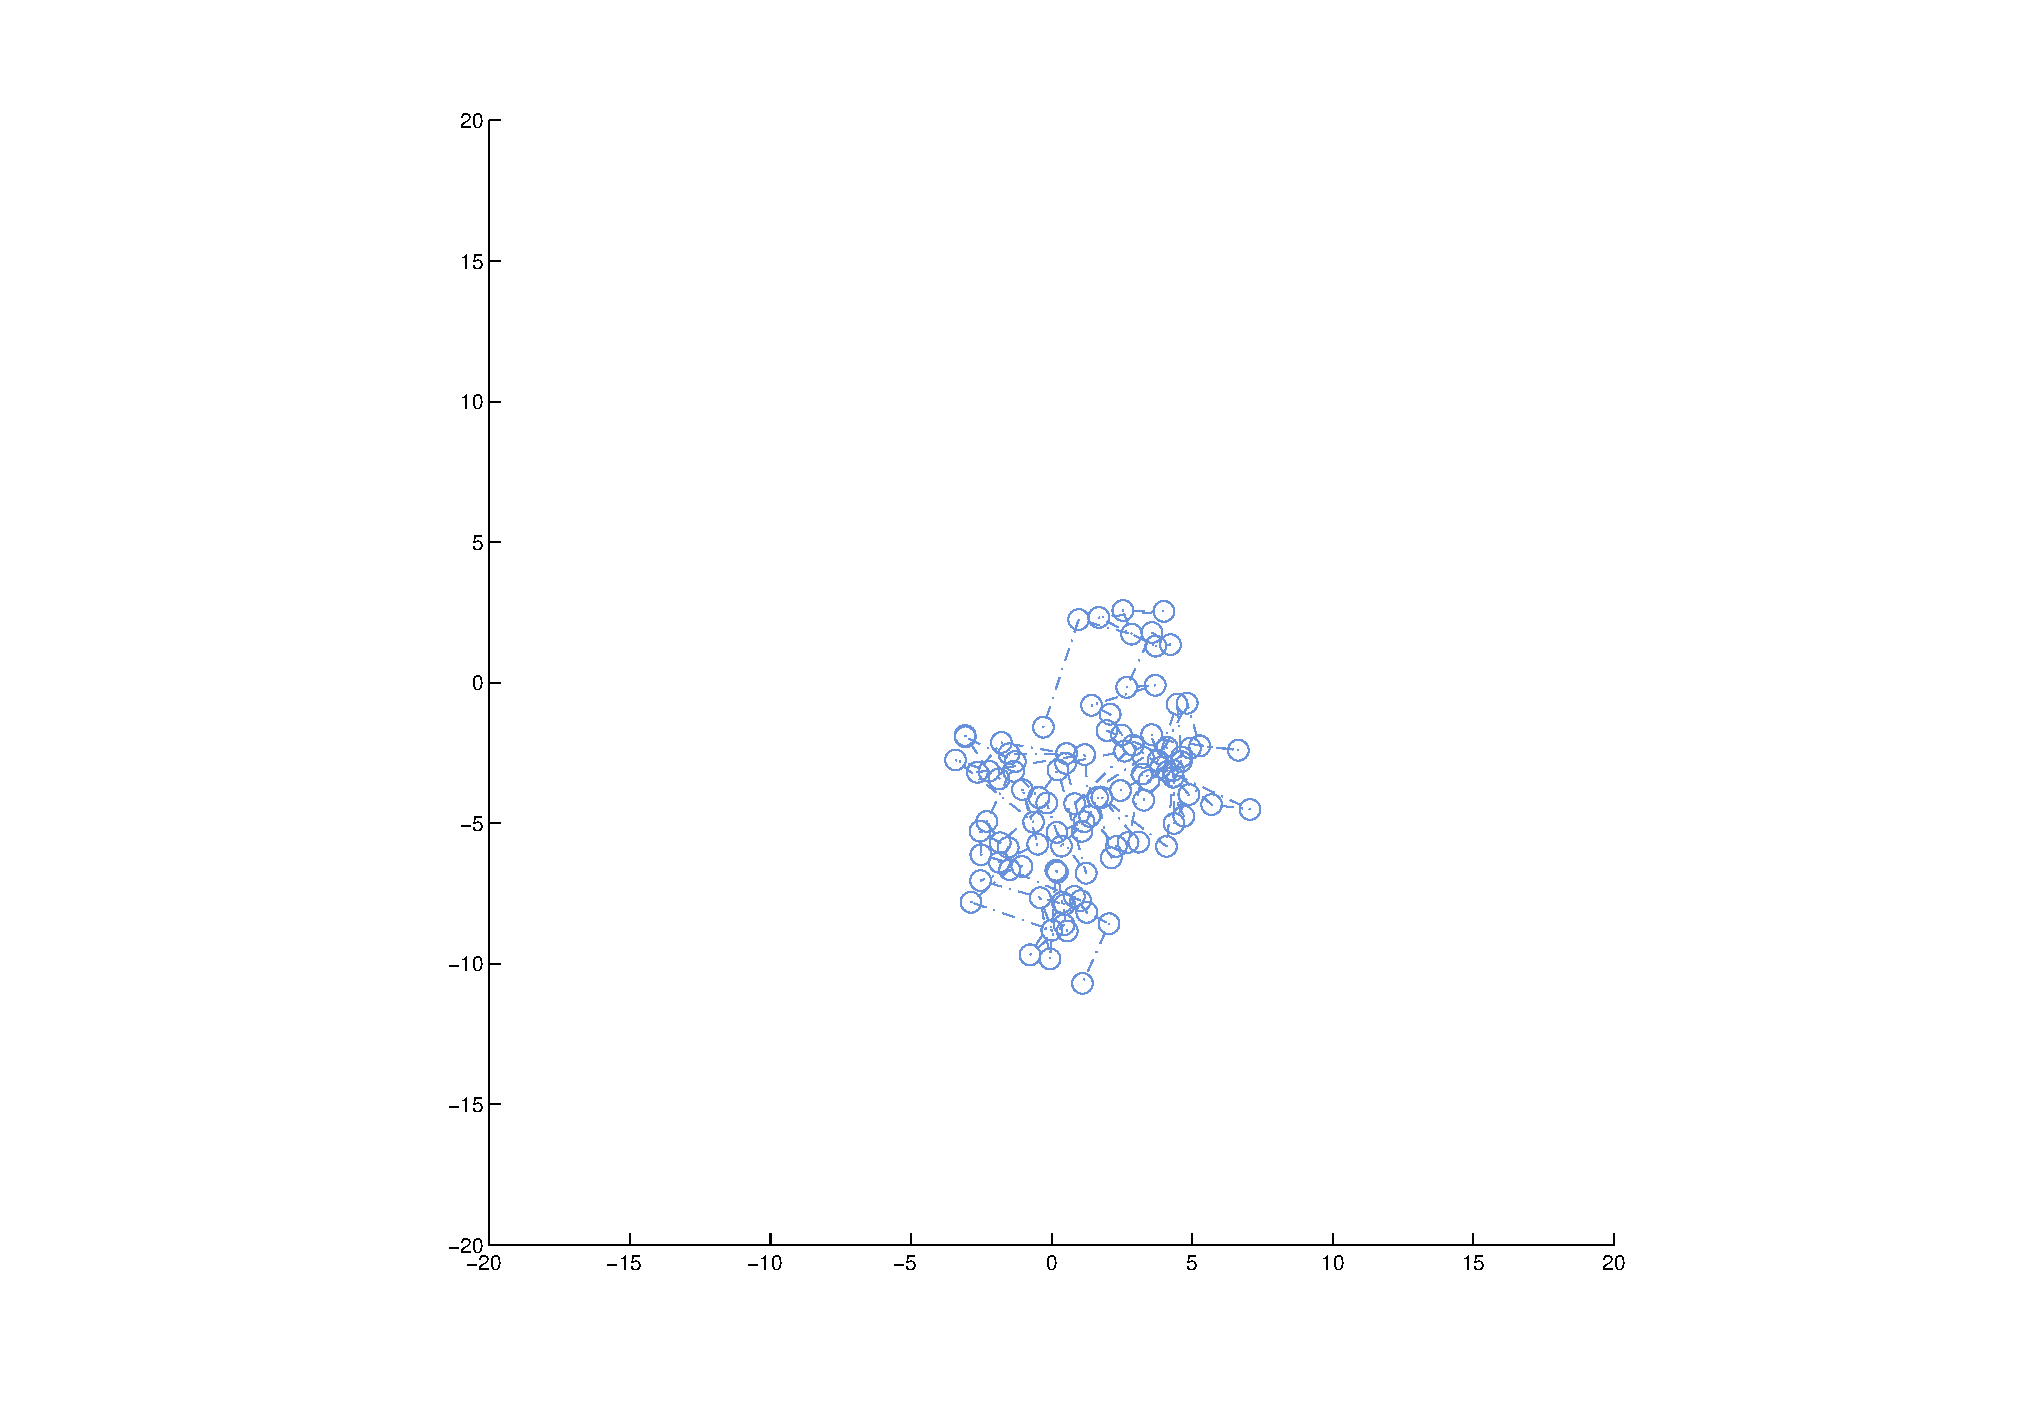
\includegraphics[width=3.2in]{1.eps}
		\caption{initial position}
	\end{minipage}%
	\begin{minipage}[t]{0.5\textwidth}
		\centering
		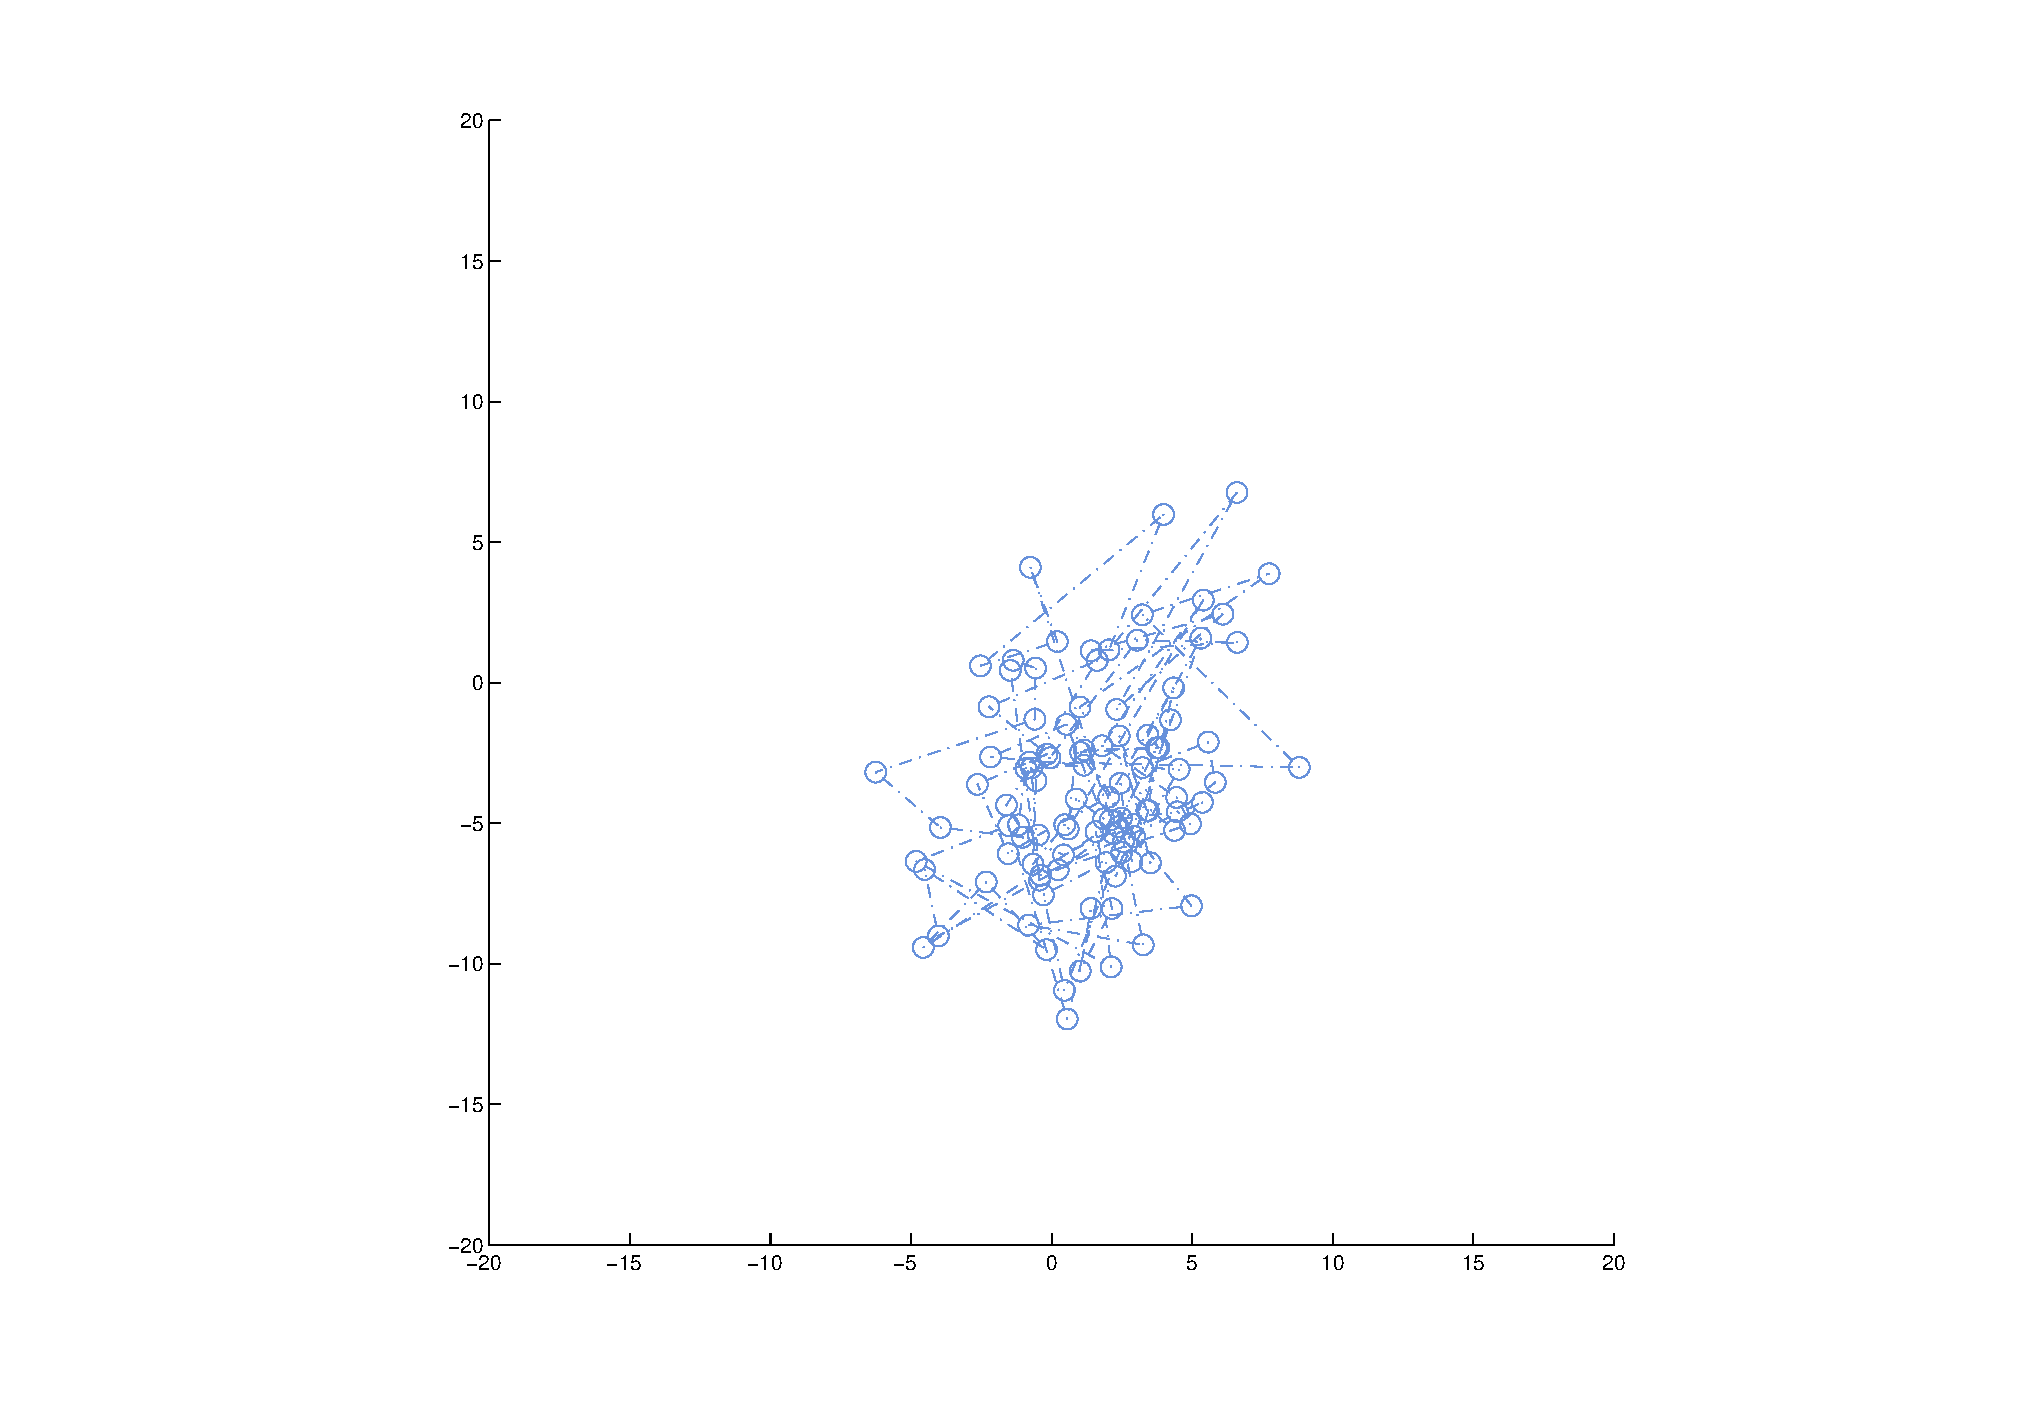
\includegraphics[width=3.2in]{2.eps}
		\caption{final position}
		
	\end{minipage}
\end{figure}
\subsection{Probability distribution function of $\bm{R}$  }
In order to verify that the PDF of $\bm{R}$ is Gaussian,we calculate the 'end to end distance' $\bm{R}$ for each simulation,then we plot it with histogram by coordinate $(x,y,z)$ respectively and compare with the probability distribution function of $\bm{R}$ in theory. 
\begin{lstlisting}
%this program is used to simulate the probability distribution of Gaussian 
classdef Idealchain<handle

properties
dimension%dimension=3
numParticles%number of particles in polymers;
dt%pas de temps
numSteps% number of motion
diffusionConst %constante diffusion
paths %the paths of polymer;
endToEndDist %end to end distance 
simulation %number of simulations
end

methods

%class constructor
function obj=Idealchain(dimension,numParticles,dt,diffusionConst,numSteps,simulation)
obj.dimension=dimension;
obj.numParticles=numParticles;
obj.dt=dt;
obj.numSteps=numSteps;
obj.diffusionConst=diffusionConst;
obj.simulation=simulation;
obj.paths = zeros(2,3,2);
obj.endToEndDist=zeros(obj.simulation,3);
end


function Calculate(obj)
for s=1:obj.simulation 
%step 1:connect the chain;
obj.paths(1,1:obj.dimension,1)=[0 0 0];%position of first beed;
obj.paths(2,1:obj.dimension,1)=obj.paths(1,1:obj.dimension,1);
noise=sqrt(2*obj.diffusionConst*obj.dt)*randn(1,obj.dimension);
for i=1:obj.numParticles
obj.paths(2,1:obj.dimension,1)=obj.paths(2,1:obj.dimension,1)+noise;%position of last beed;
end

%step 2:end :the position of beed 1 and beed end varity by time;
for j=2:obj.numSteps
obj.paths(1,1:obj.dimension,2)=obj.paths(1,1:obj.dimension,1)+noise;
obj.paths(2,1:obj.dimension,2)=obj.paths(2,1:obj.dimension,1)+noise;   
obj.paths(1,1:obj.dimension,1)=obj.paths(1,1:obj.dimension,2);
obj.paths(2,1:obj.dimension,1)=obj.paths(2,1:obj.dimension,2);  
end
obj.endToEndDist(s,:)=obj.paths(2,:,2)-obj.paths(1,:,2);


end

end

function Plot(obj)
% 
%           figure(2);
%          plot(obj.endToEndDist);

%          figure(3)
%        [h,bins]= hist(obj.endToEndDist(:,1),50);
%          bar(bins,h);
%        

f=@(N,R,b)(sqrt(1/(2*pi*N*b^2))*exp(-(sum(R.^2,2))./(2*N*b^2)));%PDF 
subplot(2,2,1)
[h, bins]=hist(obj.endToEndDist(:,1),50); h= h./sum(h); bar(bins,h),...
hold on, 
plot(bins,f(obj.numParticles,[bins'],1),'r')
title('PDF on x')

subplot(2,2,2)
[h, bins]=hist(obj.endToEndDist(:,2),50); h= h./sum(h);bar(bins,h),...
hold on, plot(bins,f(obj.numParticles,[bins'],1),'r')
title('PDF on y')

subplot(2,2,3)
[h, bins]=hist(obj.endToEndDist(:,3),50); h= h./sum(h); bar(bins,h),...
hold on, plot(bins,f(obj.numParticles,[bins'],1),'r')
title('PDF on z')
%plot(3/(2*pi*obj.numParticles*1)^1.5*exp(3*obj.R.^2/(2*obj.numParticles*1)))

end

end
end 

\end{lstlisting}
\begin{figure}[H]
	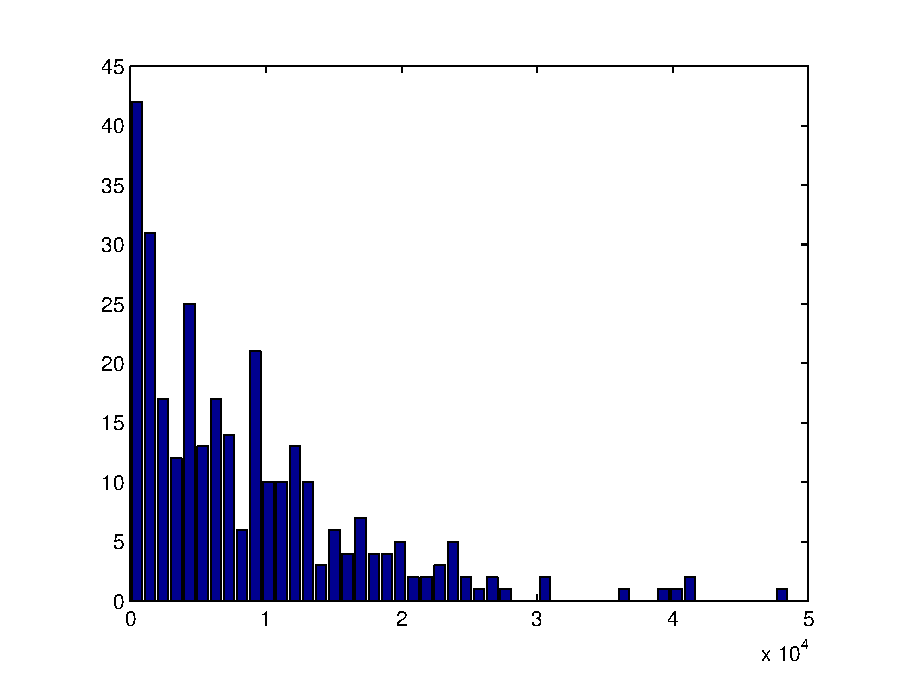
\includegraphics[width=6.2in]{MetTime3.eps} 
	 
	 \end{figure}
	 \section{The bead-spring model}
	 \paragraph{}
	 The bead-spring model is also called Rouse Model .In this model,the single chain diffusion is represented by Brownian motion ,there is no exclude volume 	interactions between the beads and each bead experience a drag force proportional to their velocity ,then the position of the beads will satisfy the Langevin equation :
	 \begin{equation}
	 \frac{d\bm{R_n}}{dt}=\frac{k}{\xi}(\bm{R_{n+1}}+\bm{R_{n-1}}-2\bm{R_{n}})+\bm{g_n}, \forall n \in [1,2...N-1]
	 \end{equation}
	 For the bead $0$ and $N$,we have :
	 \[
	 \begin{cases}
	\frac{d\bm{R_0}}{dt}=\frac{k}{\xi}(\bm{R_{1}}-\bm{R_{0}})+\bm{g_n}\\
	\frac{d\bm{R_n}}{dt}=\frac{k}{\xi}(\bm{R_{n-1}}-\bm{R_{n}})+\bm{g_n}
	 \end{cases}
	 \]
	 where $\xi$ is friction coefficient,$k$ is spring constant.
	 \subsection{Rouse Model Simulation}
	 \begin{lstlisting}
	 %This program is used to simulate the spring-bead model
	 classdef RouseModel<handle
	 properties
	 dimension%dimension=1,2 or 3
	 numParticles%number of particles in polymers;
	 dt%pas de temps
	 numSteps% number of motion
	 numSimulations%number of simulations;
	 diffusionConst %constante diffusion
	 paths %the paths of polymer;
	 frictionCoefficient;%the frictionCoefficient of a bead;
	 MetBeedNum; %the number of the beed which have met with the first and last beed;
	 connectedBeads %an n by two array with pair wise bead numbers to connect
	 fixedBeads %numBeads of beads that do not move
	 b %length between 2 beads 
	 end
	 
	 methods
	 
	 
	 function obj=RouseModel(dimension,numParticles,dt,diffusionConst,...
	 numSteps,frictionCoefficient,connectedBeads, fixedBeads,b)
	 
	 obj.dimension = dimension;
	 obj.numParticles = numParticles;
	 obj.dt = dt;
	 obj.numSteps = numSteps;
	 obj.diffusionConst = diffusionConst;
	 obj.paths = zeros(obj.numParticles,3,obj.numSteps);
	 obj.frictionCoefficient = frictionCoefficient;
	 obj.fixedBeads= fixedBeads;
	 obj.connectedBeads = connectedBeads ;
	 obj.b=b;
	 end
	 
	 
	 function Simulation(obj)
	 
	 % set initial position
	 for j=1
	 noise = [zeros(1,obj.dimension);...
	 sqrt(2*obj.diffusionConst*obj.dt)*randn(obj.numParticles-1,obj.dimension)];
	 obj.paths(:,1:obj.dimension,j)=cumsum(noise);
	 
	 end
	 
	 a = obj.dimension*obj.diffusionConst/obj.b^2;
	 R = RouseMatrix(obj.numParticles, obj.connectedBeads, obj.fixedBeads);
	 
	 for j=2:obj.numSteps
	 
	 noiseSingle = sqrt(2*obj.diffusionConst*obj.dt)*randn(obj.numParticles,obj.dimension);
	 %                 obj.paths(:,:,j)=obj.paths(1,:,j-1)+obj.dt*(a*(obj.paths(2,:,j-1)-obj.paths(1,:,j-1)))+noiseSingle;
	 
	 % zero out noise for fixed particles
	 noiseSingle(obj.fixedBeads,:) = 0;
	 
	 obj.paths(:,1:3,j) = -a*R*obj.paths(:,1:3,j-1)*obj.dt+noiseSingle +obj.paths(:,1:3,j-1);
	 
	 end
	 
	 end
	 
	 
	 function Plot(obj)
	 f=figure;
	 b=[-10 10];
	 d= axes('Parent',f,'NextPlot','replaceChildren','XLim',b,'YLim',b,'ZLim',b);
	 daspect([1 1 1]);
	 cameratoolbar
	 c=rand(1,3);
	 
	 x = obj.paths(:,1,1);
	 y = obj.paths(:,2,1);
	 z = obj.paths(:,3,1);
	 
	 l=line('XData',x,'YData',y,'ZData',z,'Color',c,'linestyle','-.','Marker','o','markersize',10,'Parent',d);
	 for i=2:obj.numSteps
	 
	 set(l,'XData',obj.paths(:,1,i),'YData',obj.paths(:,2,i),'ZData',obj.paths(:,3,i));
	 
	 pause(0.2)
	 
	 drawnow
	 end
	 
	 
	 end
	 
	 end
	 end
	 \end{lstlisting}
	 
\end{document}